\chapter{System Design}
\dictum[Antoine de Saint-Exupéry -- French writer and aviator]
{\flushright{}Grown-ups never understand anything for themselves, and it is tiresome for children to be always and forever explaining things to them.}

This chapter is about the system design of the proposed framework. The first
section will introduce the design goals of the system, which
are based on the non-functional requirements from section
\ref{non-functional-requirements}. After that, section two shows the
subsystem decomposition of the framework and the system (including the game
and the pedagogical agent). Section three shows the global control flow through
the subsystems and the last section goes into persistence of data.

%~\section{Overview}

\section{Design Goals}
This section describes a short list of design goals which are important for
the framework for several reasons. The design goals are refined from the
non-functional requirements from section \ref{non-functional-requirements}.

\subsection{Well Documented API}
The goal of the framework is to be used by as many games as possible. To reach
the goal it should have a well documented API in order to make it easy for game
developers to use the framework for their games.

\subsection{Extension Points}
Extension points give the framework the possibility to use game specific
pedagogical approaches. Clear interfaces have to be designed to support as
many different pedagogical strategies as possible. The framework should
provide extension points in form of a facade which accepts to integrate new
strategies into the framework, if they are conform to a specified interface.

\section{Subsystem Decomposition}
Figure \ref{subsystem_decomp} shows an overview of the subsystems of the
proposed framework, including the game which consists of a game engine and a
pedagogical engine, the game is not part of the framework itself but showing
them in the subsystem decomposition helps to understand the relations between the framework and the game.
The following sections will explain the dependencies between the subsystems in
detail.

\begin{figure}
    \centering
    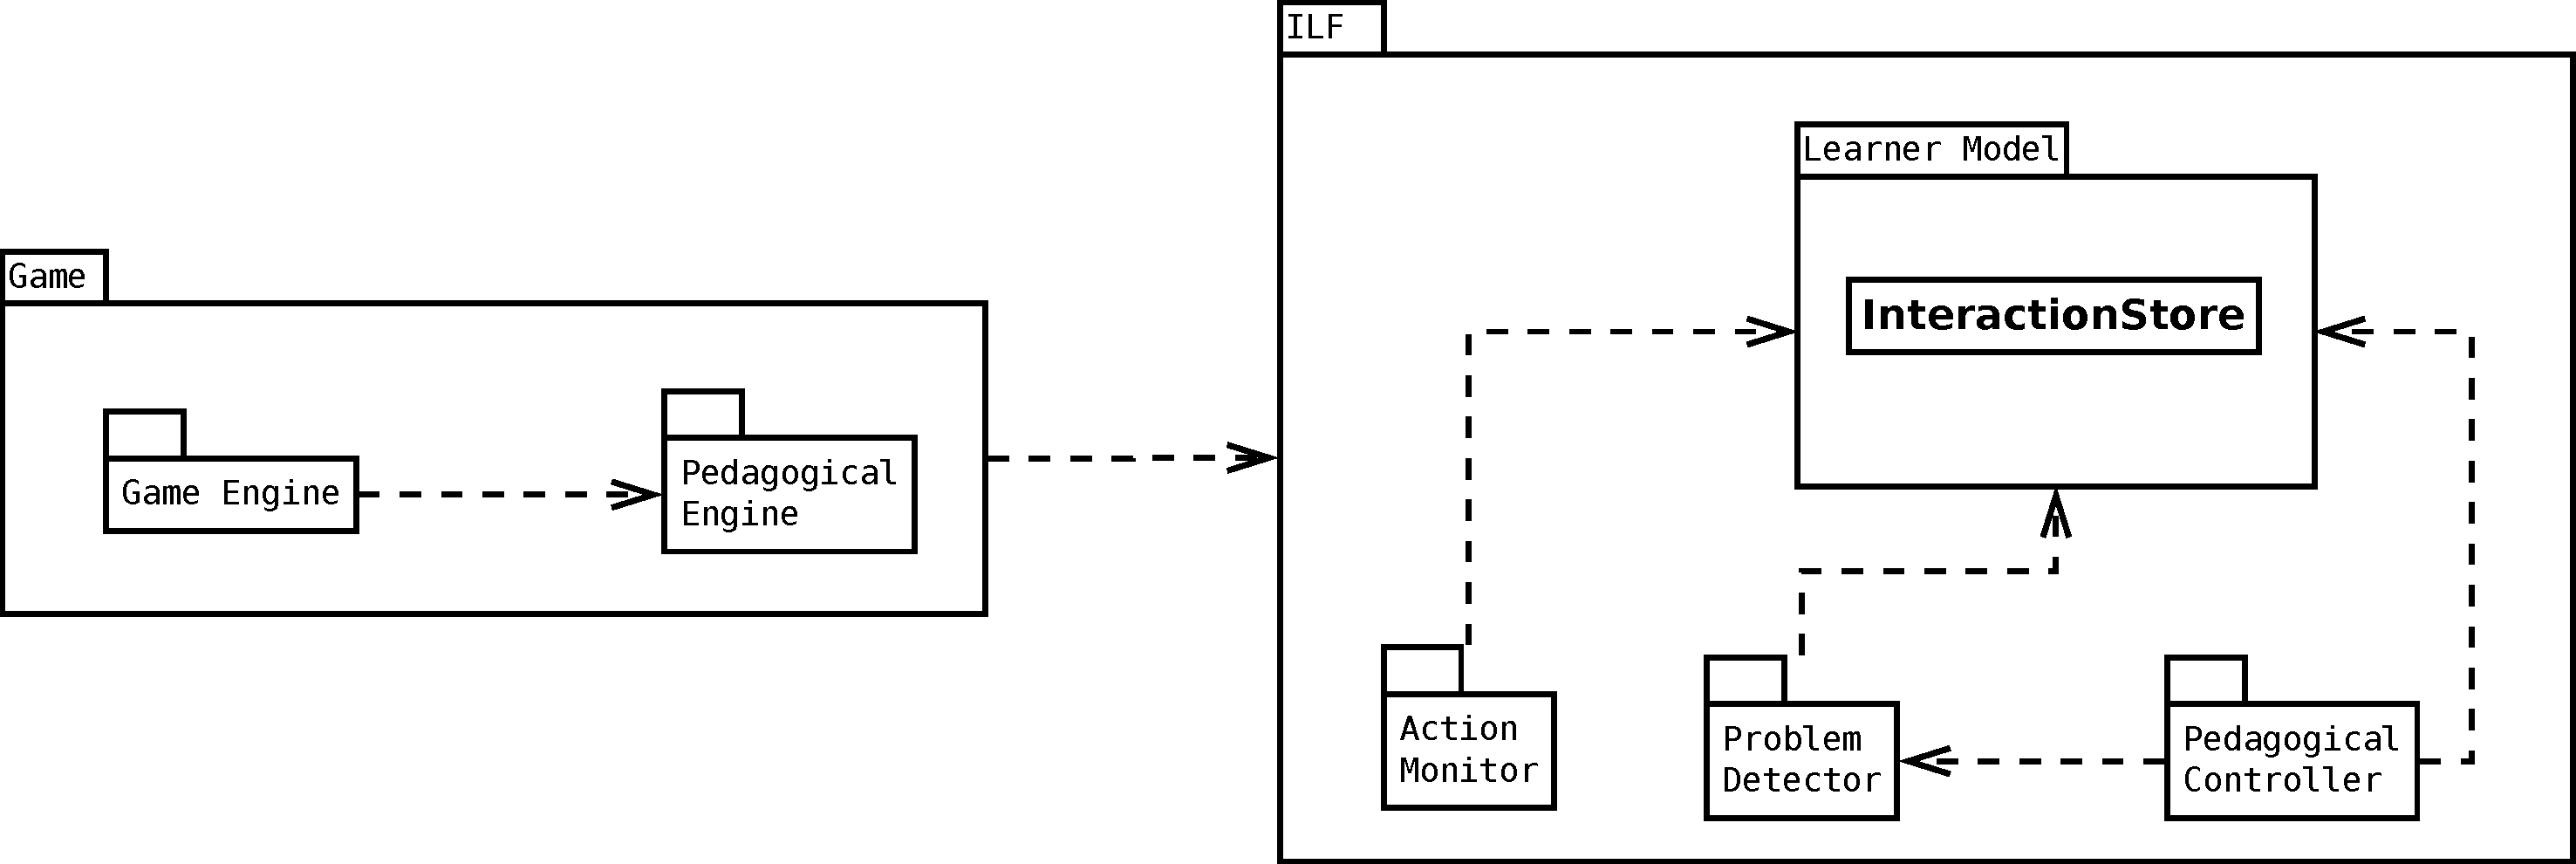
\includegraphics[width=\textwidth]{diagrams/subsystem_decomposition_new.pdf}
    \caption[Subsystem Decomposition Overview (UML package diagram)]
    {Subsystem Decomposition Overview (UML package diagram)}
    \label{subsystem_decomp}
\end{figure}

\subsection{Relation Between the Game and the Framework}
The game depends on the framework in two places: one is the \textbf{Learner}
subsystem which acts like the model in a Model-View-Controller (MVC)
architecture, the other one is the way back from the framework to the
pedagogical engine. Figure \ref{game_framework} shows the two connection points
between the game and the framework.

\begin{figure}
    \centering
    \includegraphics[width=0.6\textwidth]{diagrams/game_framework_communication.pdf}
    \caption[The Communication Interfaces between the Game and the Framework (UML package diagram)]
    {The Communication Interfaces between the Game and the Framework (UML package diagram)}
    \label{game_framework}
\end{figure}

The \textbf{Learner} subsystem contains all the models which are important to
represent the learner and his actions. This makes it the first connection point
for the \textbf{Game}. This subsystem provides the needed interfaces for the game,
so the game can notify the framework about new actions the learner performed. It
is the central part of the framework where all the important information about the learner is
stored. It makes the framework literally ``learner-centric''.

The stored actions are then interpreted by the subsystems \textbf{Action
Monitor} and \textbf{Problem Detection} which provide the main functionality
of the framework: classifying actions and interactions and detect problems. The
way back, after all the classification and problem detection is done, goes
through the \textbf{Pedagogical Controller}. The \textbf{Pedagogical Controller}
has two important jobs to do: it has to provide an interface for the game
which allows the game to add new pedagogic strategies, and it has to
provide an abstract class which the game has to implement. This
class is the \textbf{PedAgent} which should be implemented as a
\textbf{ConcretePedAgent} class in the game (see figure \ref{pedagent_concrete}).

\begin{figure}
    \centering
    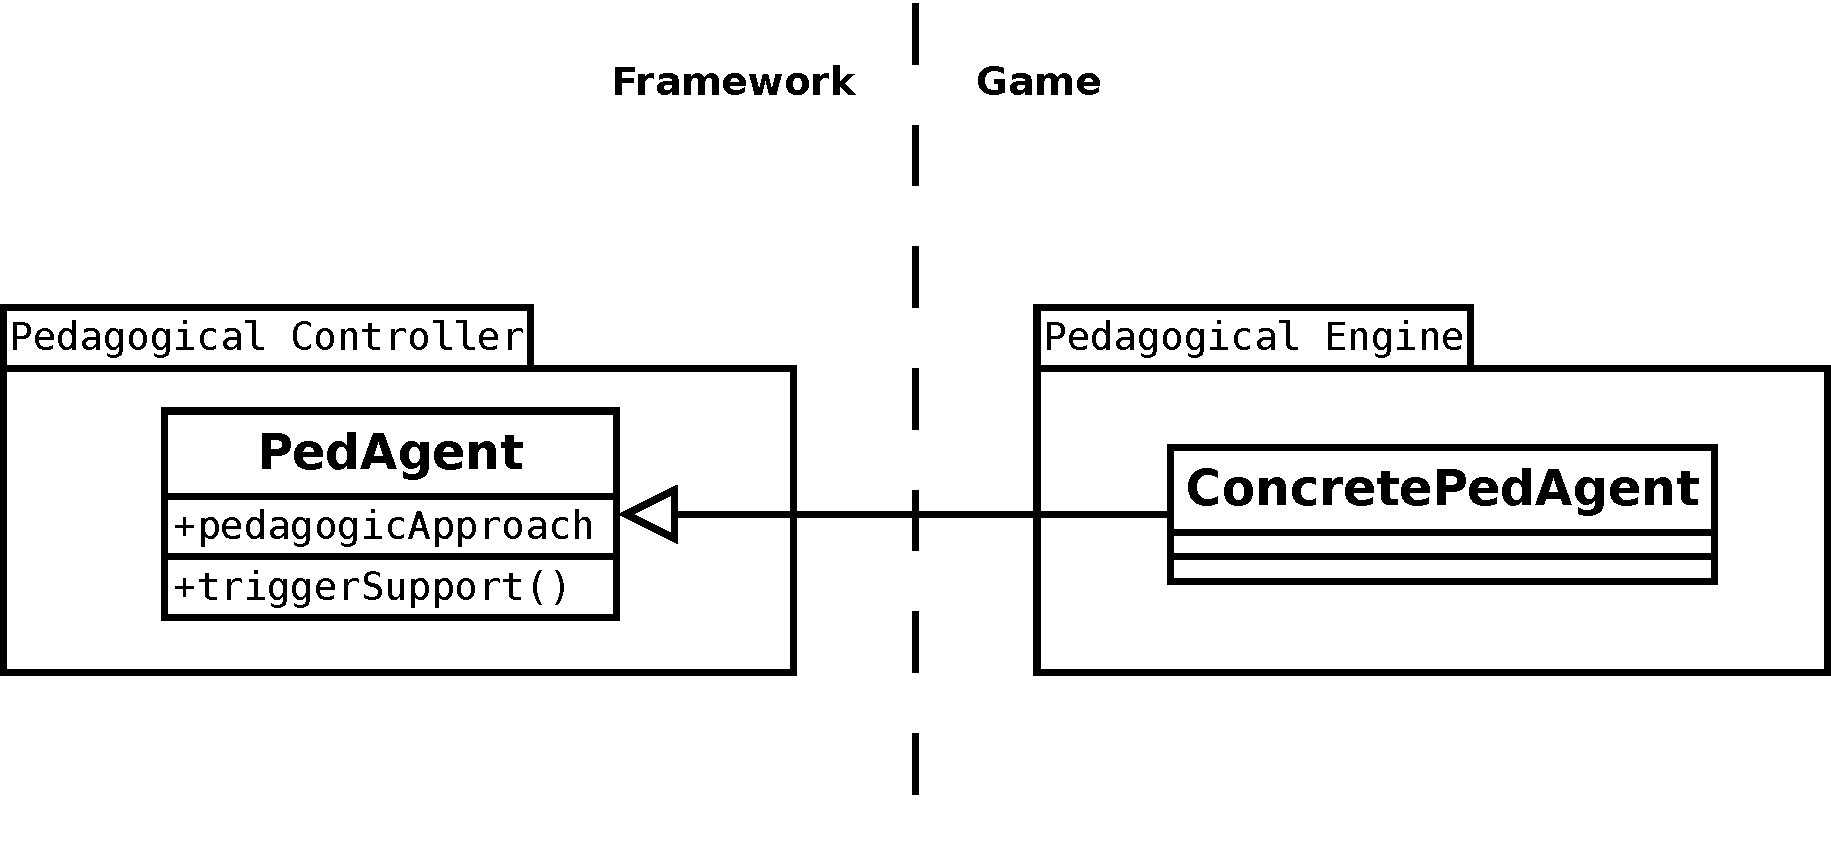
\includegraphics[width=0.6\textwidth]{diagrams/pedagent_concrete.pdf}
    \caption[The ConcretePedAgent implements the Abstract Class PedAgent (UML class diagram)]
    {The ConcretePedAgent implements the Abstract Class PedAgent (UML class diagram)}
    \label{pedagent_concrete}
\end{figure}

\subsection{The Core of the Framework}
\label{core_framework}
The previous section covered the interfaces which handle the communication between
the game and the framework. This section shows the decomposition of the core
parts of the framework.

The core of the framework can be divided into four major parts: the
\textbf{Learner}, \textbf{Problem Detector}, \textbf{Pedagogical Controller}
and \textbf{Action Monitor} subsystems. The \textbf{Learner} subsystem
summarizes all the models needed to represent the learner with his
preferences, personality aspects and so on. The interaction model is also part
of the \textbf{Learner} subsystem, because it is highly related to the learner.
The \textbf{Learner} subsystem also provides the essential interfaces to
communicate with the game, as already mentioned in the last section.

%~a central place in the framework
%~where information is stored and can be accessed. In a classic
%~Model-View-Controller (MVC) architecture, the \textbf{Learner} would be the model.

%~The \textbf{Action Monitor} subsystem provides an interface for the game to
%~communicate with the framework about new actions. The game sends these actions
%~continuously to the \textbf{Action Monitor}. The \textbf{Action Monitor}
%~evaluates the actions performed and identifies interactions which are then
%~stored in the interaction model. The \textbf{Action Monitor} has the job to
%~monitor actions which occurred in the game and classify them into higher level
%~objects: interactions.

The \textbf{Action Monitor} works like a factory: actions come in as raw
material on one side, get processed, grouped and classified and come out on the
other side as interactions, which are stored in the \textbf{Learner}
subsystem. To do so, the \textbf{Action Monitor} has to subscribe to the
\textbf{Learner} subsystem which notifies it when new actions have been
performed by the \textbf{Learner}.

%~Figure \ref{action_monitor} shows the
%~\textbf{Action Monitor} and the interfaces it provides and uses
%~in a component diagram.

%~\begin{figure}
    %~\centering
    %~\includegraphics[width=\textwidth]{diagrams/action_monitor.pdf}
    %~\caption[Component diagram of the Action Monitor]
    %~{Component diagram of the Action Monitor}
    %~\label{action_monitor}
%~\end{figure}

The subsystem \textbf{Problem Detector} is responsible for recognizing
problems during the learning process. This subsystem depends on the
\textbf{Learner} subsystem, where the interactions are stored. The problem
detection listens to all the interactions and gets notified when new
interactions have happened. Doing so, the subsystem is always on track and can
examine the recent history of interactions. The magic of the subsystem lies in
a matching method, which matches interaction patterns to problems. This makes
it the perfect point to introduce artificial intelligence in problem
recognition, which will be discussed in the future work chapter at the end of
this thesis (see chapter \ref{future_work}).

Last but not least the \textbf{Pedagogical Controller} subsystem, which depends
on the \textbf{Learner} subsystem (because it needs to be aware of all the
learner specific information, e.g. preferences) and on the
\textbf{Problem Detector} subsystem (which informs the \textbf{Pedagogical
Controller} about problems which might have occurred). This subsystem features
the full pedagogical knowledge which the framework brings with it and offers
an API to add additional pedagogic strategies. The \textbf{Pedagogical
Controller} is the brain of the pedagogical agent which has to be implemented
as part of the game itself (outside the framework).

\section{Global Control Flow}
Figure \ref{control_flow} shows an exemplary flow of events through the
different subsystems. Although the \textbf{Game} is an external system and not
part of the framework, it has its own lifeline, because it is highly related
to the framework and helps to understand the global control flow. For now, the
lifelines represent subsystems (except the \textbf{InteractionStore}
which is part of the \textbf{Learner} subsystem) and will be refined later into
entity, control and boundary objects.

The first step in the global control flow is when the \textbf{Learner} starts
to play the \textbf{Game}. The \textbf{Game} records the actions of the
\textbf{Learner} and forwards them to the \textbf{Action Monitor}, which
starts to classify the actions into larger groups of actions: interactions. The
interactions are stored in the \textbf{Learner} subsystem, to be more precise in the
\textbf{InteractionStore}, which is only one part of the \textbf{Learner}
subsystem. The next step in the flow of events is triggered by the newly
created interaction: the \textbf{Problem Detector} subsystem is notified
about the new interaction and determines whether this leads to a problem or
not. In the global control flow shown in figure \ref{control_flow}, a case is
modeled where an actual problem occurred. The \textbf{Problem Detector} notifies
the \textbf{Pedagogical Controller} about a new problem. The controller
determines which support strategy is the best considering the learners
personality, learning history and the type of problem. Now is the time for the
pedagogical agent to step in and support the learner in order to resolve their
problem.

\begin{figure}
    \centering
    \includegraphics[width=\textwidth]{diagrams/global_control_flow_new.pdf}
    \caption[The Global Control Flow through the Subsystems (UML sequence diagram)]
    {The Global Control Flow through the Subsystems (UML sequence diagram)}
    \label{control_flow}
\end{figure}

\section{Persistent Data}
This section lists in short the parts of the framework which have to be
persistent. These parts are identified easily, because all the information of
the learner needs to be persistent for future use. The learners preferences,
personality aspects and of course the learners actions determine the behavior
of the learner. It is also important to store the complete
learning history of the learner (every action and interaction, every problem),
because the information can be used later to evaluate and improve the
framework and its detection and adaptation approaches.

At the bottom line: The \textbf{Learner} subsystem needs to keep its
information about the learner persistent. There may appear some more
persistent objects during the object design, which will persist their contents
too if there is need to. For more details see Chapter \ref{object_design}:
Object Design.
